%%%%%%%%%%%%%%%%%%%%%%%%%%%%%%%%%%%%%%%%%%%%%%%%%%%%%%%%%%%%%%%%%
%  _____       ______   ____									%
% |_   _|     |  ____|/ ____|  Institute of Embedded Systems	%
%   | |  _ __ | |__  | (___    Wireless Group					%
%   | | | '_ \|  __|  \___ \   Zuercher Hochschule Winterthur	%
%  _| |_| | | | |____ ____) |  (University of Applied Sciences)	%
% |_____|_| |_|______|_____/   8401 Winterthur, Switzerland		%
%																%
%%%%%%%%%%%%%%%%%%%%%%%%%%%%%%%%%%%%%%%%%%%%%%%%%%%%%%%%%%%%%%%%%

\chapter{Metastabilität}\label{chap.metastabilitat}

\section{Definition Metastabilität}\label{sect.meatastabil_def}
Metastabilität bedeutet, dass der Ausgang eines Flip-Flops nicht dem Eingang entsprechen muss. Wechselt das Inputsignal eines Flip-Flops zur falschen Zeit, ist der Wert des Ausgangssignal unsicher. Hier zwei kurze englische Beschreibungen, dieses Phänomens:\\
\newline
'' If data inputs to a flip-flop are changing at the instant of the clock pulse, a problem known as \textit{metastability} may occur. In the metastable case, the flip-flop does not settle in to a stable state'' (Camara, S. 32-2)  \\
\newline
''If the amplitude of the runt pulse is \textit{exactly the treshold level of the SET input of the output cell}, the cell will be driven to its metastable state. The metastable state is the condition that is roughly defined as ''half SET and half RESET'' (Fletcher, 482.)\\
\newline
\\
Im besten Fall wählt der Ausgang bei unklarem Eingangssingal selbst einen Wert an ('0' oder '1'). Im schlechten Fall “hängt” sich das Flip-Flop “auf” und toggelt permanent zwischen '0' und '1' oder setzt sogar beide Werte parallel.

\begin{figure}[H]
	\centering
	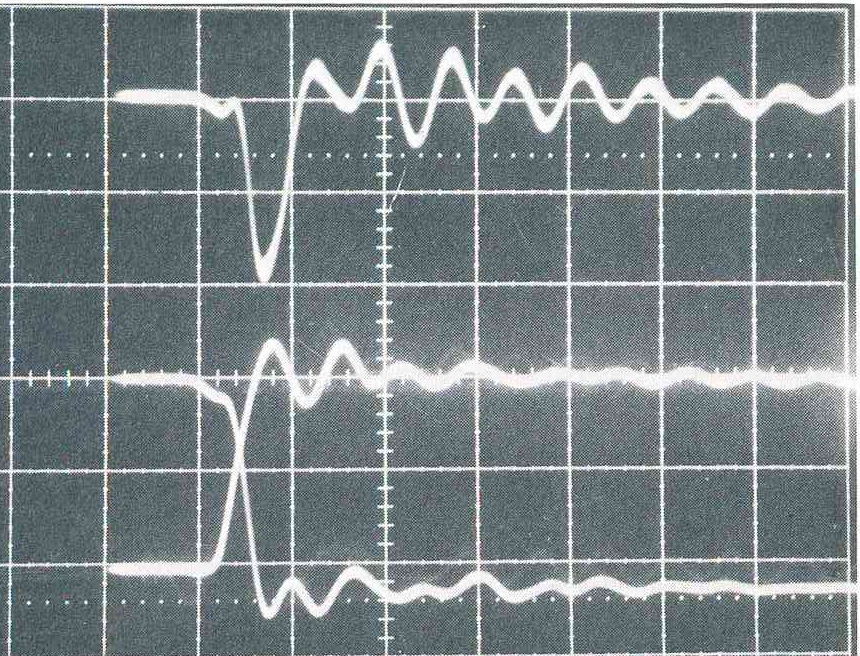
\includegraphics[width=0.4\textwidth]{images/metastability/metastability_2_IO.png}
	\caption{Metastabilität schlimmster Fall (Fletcher, 482.)}
	\label{fig.metastabil.schlimmster_Fall}
\end{figure}


\section{Ursache von Metastabilität}\label{sect.meatastabil_ursache}
Der Grund für Metastabilität ist, dass der angelgte Wert entweder zu spät eintrifft (verletzen der setup-Zeit) oder zu früh wieder verschwindet (verletzen der hold-Zeit). Metastabilität kann vermieden werden, wenn diese zwei Zeiten strikt eingehalten werden:\\
\newline
''Metastabilit is avoided by holding the information stable before and after the clock pulse  for a set period of time, called the setup time for the data line an the hold time for the control line.''(Camara, S. 32-2)
\begin{figure}[H]
	\centering
	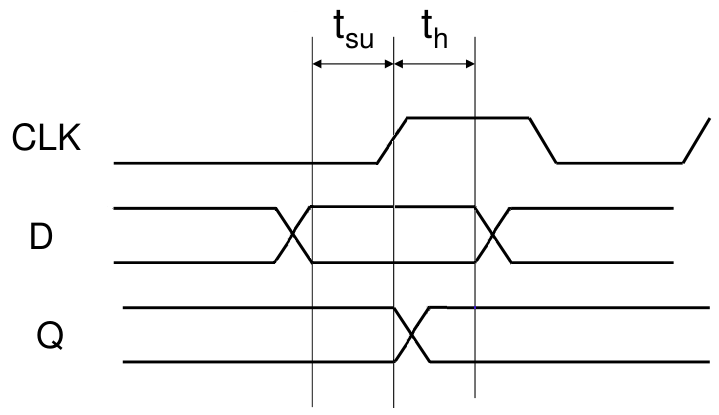
\includegraphics[width=0.4\textwidth]{images/metastability/kritscheZeit_FF.png}
	\caption{Einhalten der Datenzeiten}
	\label{fig.metastabil.kritisches_zeitfenster}
\end{figure}
Es gibt mehrere Gründe für das Nichteinhalten der geforderten setup-Zeit:\\
- Ein Logikpfad kann zu lange sein, bzw. die Taktfrequenz ist zu schnell\\
- Zwischen den Bauteilen liegen zu lange Pfade, die das Eintreffen der Daten verzögern\\
- Ein vorangehendes Bauteil hat eine zu lange Durchlaufverzögerung.\\
\\
Um Metastabilität zu vermeiden, sollte die Logik möglichst klein gehalten werden, die Bauteile bewusst nahe beieinander platziert und vor allem der Systemtakt an die längste Pfadzeit angepasst werden. Der maximal elaubte Systemtakt kann in quartus mit dem Timequest Time Analyser abgefragt werden.\\
Als Alternative bietet sich eine Synchronisierungsschaltung an. Zwischen den zwei Takt-Flanken kann sich der metastabile Ausgang erholen und gelangt so stabil in den Verarbeitungspfad. Der Nachteil der Synchronistation ist jedoch, eine um einen Takt längere Verarbeitungszeit.\\


\section{Metastabilität erzeugen}\label{sect.meatastabil_erzeugen}
\subsection{Ansatz}\label{sect.metastabil_ansatz}
Aufgebaut wird ein System mit zwei Takten. Der zentrale Block hat eine Taktfrequenz von 50 MHz und beinhaltet eine State Machine. Diese wechselt bei jedem Impuls von einem Zustand in den anderen (Abbild: \ref{fig.metastabil.statemachine} Um die zwei Zustände zu erkennen, werden beiden Zuständen ein logischer Pegel zugefügt:\\
\newline
- Zustand 1:  s0  = Logisch '0'\\
- Zustand 2:  s1  = Logisch '1'\\

\begin{figure}[H]
	\centering
	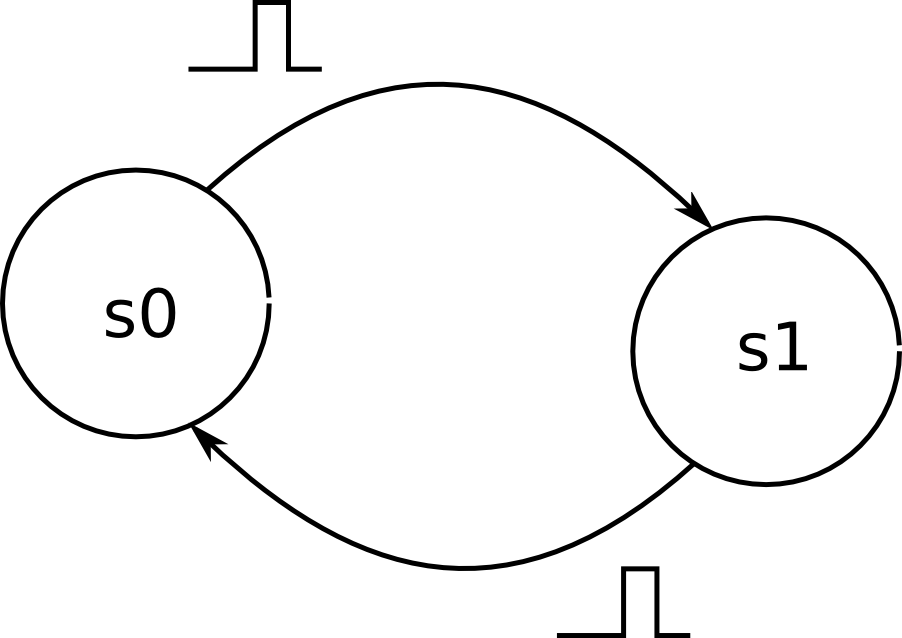
\includegraphics[width=0.2\textwidth]{images/metastability/statemachine_s0_s1.png}
	\caption{Statemachine im zentralen Block}
	\label{fig.metastabil.statemachine}
\end{figure}

Der Inpuls, der die Statemachine steuert ist asynchron. Er wird von einem Zähler generiert, der mit der Taktfrequenz von 27 MHz läuft. Alle 37 ns sendet der Zähler einen Puls an die State Machine. Die State Machine selbst arbeitet mit einer Taktfrequenz von 20 ns. Der Impuls ist ihr gegenüber asynchron.\\
\newline
Erwartet wird, dass die setup-Zeit der State Machine-Flip-Flops regelmässig verletzt werden. \\

\begin{figure}[H]
	\centering
	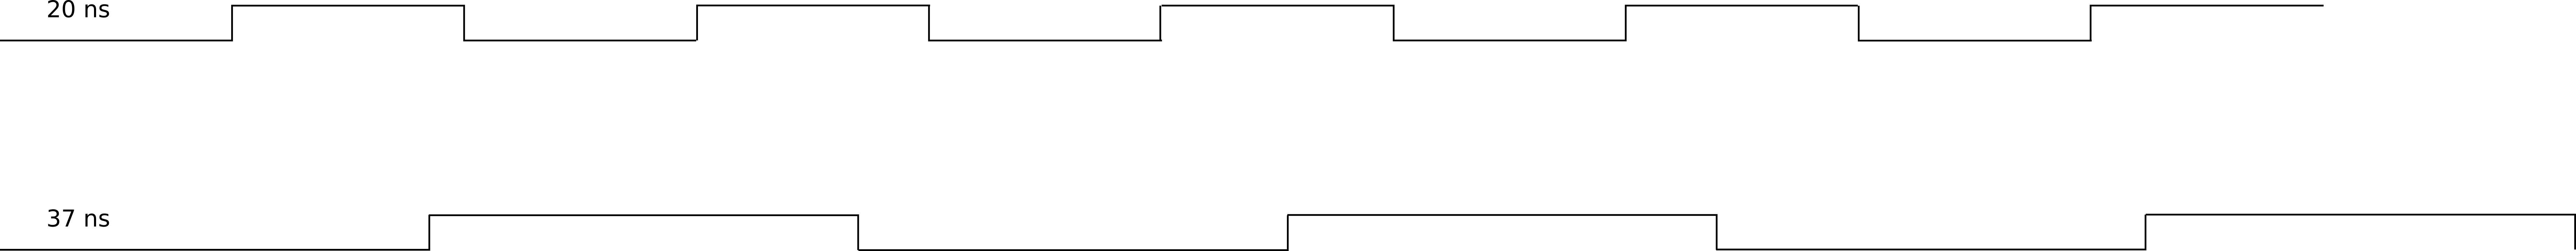
\includegraphics[width=0.2\textwidth]{images/metastability/2_takte.png}
	\caption{Die zwei Taktzeiten}
	\label{fig.metastabil.statemachine}
\end{figure}
\todo{ einsetzen setup zeit gemäss glossar für ..}


\subsection{Implementation}\label{sect.metastabil_implementation}


\section{Resultat Metastabilität provozieren}\label{sect.meatastabil_proozieren}
\textbf{Was ist das Ergebnis beim Verletzen der setup Zeit?}
Beide Ausgänge immer an?
Keiner von beiden?
aufhängen des Systems? (Keine LED geht mehr).

\textbf{Synchronisation Schaltung erhärtet die These b\\}
